\documentclass{article}
\usepackage[a4paper, portrait, margin=1.1811in]{geometry}
\usepackage[english]{babel}
\usepackage[utf8]{inputenc}
\usepackage[T1]{fontenc}
\usepackage{helvet}
\usepackage{etoolbox}
\usepackage{graphicx}
\usepackage{titlesec}
\usepackage{caption}
\usepackage{booktabs}
\usepackage{xcolor} 
\usepackage[colorlinks, citecolor=cyan]{hyperref}
\usepackage{caption}
\usepackage{tikz-qtree}
\usepackage{latexsym}
\captionsetup[figure]{name=Figure}
\graphicspath{ {./images/} }
\usepackage{scrextend}
\usepackage{fancyhdr}
\usepackage{graphicx}
\newcounter{lemma}
\newtheorem{lemma}{Lemma}
\newcounter{theorem}
\newtheorem{theorem}{Theorem}

\fancypagestyle{plain}{
	\fancyhf{}
	\renewcommand{\headrulewidth}{0pt}
	\renewcommand{\familydefault}{\sfdefault}
}

%\pagestyle{plain}
\makeatletter
\patchcmd{\@maketitle}{\LARGE \@title}{\fontsize{16}{19.2}\selectfont\@title}{}{}
\makeatother

\usepackage{authblk}
\renewcommand\Authfont{\fontsize{10}{10.8}\selectfont}
\renewcommand\Affilfont{\fontsize{10}{10.8}\selectfont}
\renewcommand*{\Authsep}{, }
\renewcommand*{\Authand}{, }
\renewcommand*{\Authands}{, }
\setlength{\affilsep}{2em}  
\newsavebox\affbox
\author{\textbf{Olteanu Fabian Cristian}}
\affil{FMI, AI Master, Year 1
}

\titlespacing\section{0pt}{12pt plus 4pt minus 2pt}{0pt plus 2pt minus 2pt}
\titlespacing\subsection{12pt}{12pt plus 4pt minus 2pt}{0pt plus 2pt minus 2pt}
\titlespacing\subsubsection{12pt}{12pt plus 4pt minus 2pt}{0pt plus 2pt minus 2pt}


\titleformat{\section}{\normalfont\fontsize{10}{15}\bfseries}{\thesection.}{1em}{}
\titleformat{\subsection}{\normalfont\fontsize{10}{15}\bfseries}{\thesubsection.}{1em}{}
\titleformat{\subsubsection}{\normalfont\fontsize{10}{15}\bfseries}{\thesubsubsection.}{1em}{}

\titleformat{\author}{\normalfont\fontsize{10}{15}\bfseries}{\thesection}{1em}{}

\title{\textbf{\huge Knowledge Representation and Reasoning Project 1}}
\date{}    

\begin{document}

\pagestyle{headings}	
\newpage
\setcounter{page}{1}
\renewcommand{\thepage}{\arabic{page}}


	
\captionsetup[figure]{labelfont={bf},labelformat={default},labelsep=period,name={Figure }}	\captionsetup[table]{labelfont={bf},labelformat={default},labelsep=period,name={Table }}
\setlength{\parskip}{0.2em}
	
\maketitle
	
\noindent\rule{15cm}{0.4pt}

\section{Resolution}
Let us consider the following knowledge base:


KB
$\left\{
\begin{tabular}{p{.8\textwidth}}
\begin{enumerate}
		\item Every DOTA2 player is a gamer.
		\item There are DOTA2 players who are professional.
		\item Some professional DOTA2 players who purchase Divine Rapier lose games.
		\item Anyone who loses games gets angry.
\end{enumerate}
\end{tabular}
\right.$

We want to prove that the following Question is logically entailed from our KB by applying the Resolution algorithm:

\centerline{5. Do some gamers who purchase Divine Rapier get angry?} 

\subsection{Representing the KB in FOL (a)}
The above written KB can be expressed in FOL in the following way:

KB
$\left\{
\begin{tabular}{p{.8\textwidth}}
\begin{enumerate}
		\item $\forall x. DOTA2\_Player(x) \supset Gamer(x)$
		\item $\exists x. DOTA2\_Player(x) \land Pro(x)$
		\item $\exists x. PRO(x) \land Buys\_Rapier(x)\land Loses\_Games(x)$
		\item $\forall x. Loses\_Games(x) \supset Gets\_Angry(x)$
		\item $\exists x. Gamer(x) \land Buys\_Rapier(x) \land Gets\_Angry(x)$.
\end{enumerate}
\end{tabular}
\right.$

For the sake of simplicity, we can write it in the following way: 

KB
$\left\{
\begin{tabular}{p{.8\textwidth}}
\begin{enumerate}
		\item $\forall x. P_1(x) \supset P_2(x)$
		\item $\exists x. P_1(x) \land P_3(x)$
		\item $\exists x. P_3(x) \land P_4(x)\land P_5(x)$
		\item $\forall x. P_5(x) \supset P_6(x)$
		\item $\exists x. P_2(x) \land P_4(x) \land P_6(x)$.
\end{enumerate}
\end{tabular}
\right.$

\subsection{Proving manually that the Question is logically entailed from the KB (b)}
In order to apply the resolution algorithm, we must first transform the KB written in FOL in the conjunctive normal form (CNF), after which the following transformation happens:

CNF
$\left\{
\begin{tabular}{p{.8\textwidth}}
\begin{enumerate}
		\item $\neg P_1(x) \lor P_2(x)$
		\item $P_1(V)$
		\item $P_3(V)$
		\item $P_4(V)$
		\item $P_5(V)$
		\item $\neg P_5(x) \lor P_6(x)$
		\item $P_2(V) \land P_4(V) \land P_6(V)$,
\end{enumerate}
\end{tabular}
\right.$

where V is a Skolem constant (we now have seven members in the list because we can "divide" into individual items logical sequences like number 2 from the last page: $P_1(x) \land P_3(x)$ becomes 2. $P_1(x)$ and 3. $P_3(x)$). 

Lastly, we need to prove that the negated form of the question that we want to prove is logically entailed from our KB is not satisfiable. After negating, our converted KB looks like this:

CNF
$\left\{
\begin{tabular}{p{.8\textwidth}}
\begin{enumerate}
		\item $\neg P_1(x) \lor P_2(x)$
		\item $P_1(V)$
		\item $P_3(V)$
		\item $P_4(V)$
		\item $P_5(V)$
		\item $\neg P_5(x) \lor P_6(x)$
		\item $\neg P_2(V) \lor \neg P_4(V) \lor \neg P_6(V)$.
\end{enumerate}
\end{tabular}
\right.$
\begin{center}
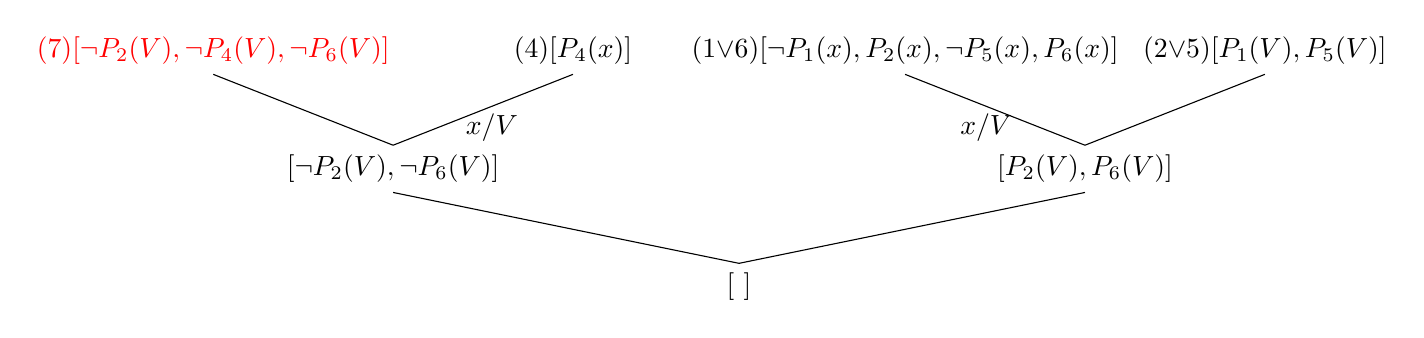
\begin{tikzpicture}[
  grow'=up,
  level 1/.style={sibling distance=25em},
  level 2/.style={sibling distance=13em}]
\node (f) {[ ]} 
child { node (1l) {$[\neg P_2(V),\neg P_6(V)]$}
  child {node (2ll) {\color{red}$(7)[\neg P_2(V),\neg P_4(V),\neg P_6(V)]$}}
  child {node (2lr) {$(4)[P_4(x)]$}}
}
child {node (1r) {$[P_2(V), P_6(V)]$}
child {node (2rl) {(1$\lor$6)$[\neg P_1(x),P_2(x),\neg P_5(x), P_6(x)]$}}
child {node (2rr) {(2$\lor$5)$[P_1(V),P_5(V)]$}}
};

   \begin{scope}[nodes = {draw = none}]
      \path (1l) -- (2lr) node [near start, right]  {$x/V$};
      \path (1r) -- (2rl) node [near start, left] {$x/V$};
   \end{scope}
\end{tikzpicture}
\end{center}

Thus, we have proven that the negated form of sentence 5 is unsatisfiable given our KB. In conclusion, the sentence: "Some gamers who purchase Divine Rapier get angry" is logically entailed from our KB. 
\end{document}